\documentclass{standalone}
\usepackage{tikz}
\usepackage{amsmath}
\renewcommand{\familydefault}{\sfdefault}


\begin{document}

\def\d{6.5}
\begin{tikzpicture}
    \node at (0*\d, 0) {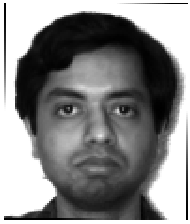
\includegraphics{../python/ex00.png}};
    \node at (1*\d, 0) {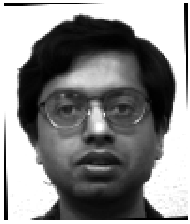
\includegraphics{../python/ex01.png}};
    \node at (2*\d, 0) {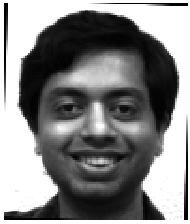
\includegraphics{../python/ex02.png}};
    \node at (3*\d, 0) {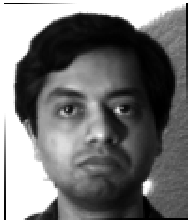
\includegraphics{../python/ex03.png}};
    \node at (4*\d, 0) {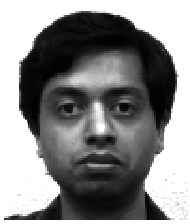
\includegraphics{../python/ex04.png}};
    \node at (5*\d, 0) {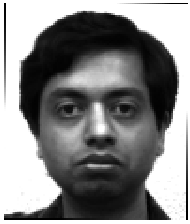
\includegraphics{../python/ex05.png}};

    \begin{scope}[yshift = -9 cm , xshift = 3.5cm]
        \node at (0*\d, 0) {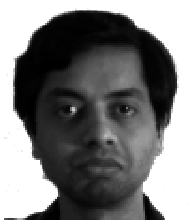
\includegraphics{../python/ex06.png}};
        \node at (1*\d, 0) {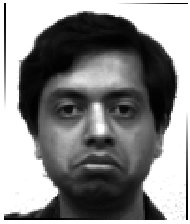
\includegraphics{../python/ex07.png}};
        \node at (2*\d, 0) {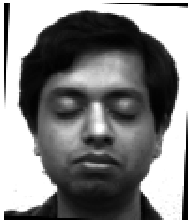
\includegraphics{../python/ex08.png}};
        \node at (3*\d, 0) {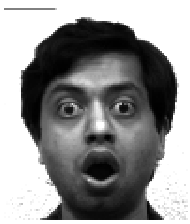
\includegraphics{../python/ex09.png}};
        \node at (4*\d, 0) {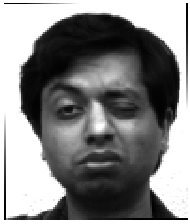
\includegraphics{../python/ex10.png}};
        
    \end{scope}

\end{tikzpicture}
% End of code
\end{document}
